\chapter{Flujometrías}
%
% El simulador ICESym requiere de información sobre el coeficiente de descarga
% (Cd) para simular el flujo a través de los puertos, en trabajos anteriores se
% realizaron simulaciones computacionales del motor con valores de Cd estimados
% \cite{lopez13}.
%
Para obtener una mejor caracterización del funcionamiento de los puertos de
admisión y escape es necesario tener mayor conocimiento del coeficiente de
descarga para para una deferentes posiciones del rotor y velocidades de giro
del motor.
%
Con este objetivo se realizaron una serie de flujometrías para obtener un mapa
de Cd en función de una diferencia de presión y alzada válvula \footnote{ICESym
utiliza alzada, por lo que se traduce área de pasaje de puerto en alzada de
válvula equivalente.}, de modo que $Cd = f(\Delta P,lv)$.
%
Este mapa de $C_D$ se usa en ICESym para obtener una simulación más precisa del
motor.

Se realizarán las flujometrías con el \emph{software} libre \emph{OpenFoam},
con los módulos \emph{pimleFoam} cuando el flujo se pueda asumir como
incompresible ($Ma < 0.3$) y \emph{rhoPimpleFoam} para flujo compresible.

Para modelar la turbulencia se utilizó un modelo de dos ecuaciones, esto porque
son modelos completos, es decir proveen una ecuación para calcular $\kappa$ y
la escala de longitud turbulenta $l$, parten de la aproximación de Boussinesq y
la ecuación de energía cinética turbulenta.

En todos los casos se utilizó el modelo de \emph{k-epsilon}, es uno de los
modelos más utilizados por su robustez y buenos resultados para números de
Reynodls bajos y diferencias de presión relativamente bajas\cite{wilcox}
%
El modelo requiere que se aproximen los valores iniciales de $\kappa$ y
$\epsilon$, que a su vez requieren de una estimación de la longitud de mezcla o
escala de la viscosidad $l_m$.
%
Los valores iniciales se calculan a partir de:

\begin{align}
    %
    C_{\mu}  &= 0.09 \\
    %
    I        &= 0.05 \\
    %
    L_m      &= 0.07 \cdot D_m \\
    %
    \kappa   &= 1.5 \cdot \left( u_{ref} \cdot I \right) ^ 2 \\
    %
    \epsilon &= \frac{C_\mu ^{3/4} \cdot \kappa ^{3/2}} {l_m}
    %
\end{align}

Dónde:
%
\begin{description}
    \item[$C_{\mu}$] es un coeficiente propio del modelo.
        %
    \item[I] es la intensidad de turbulencia estimada, en este trabajo se utilizó 0.05.
        %
    \item[$l_m$] es la longitud de mezcla o escala de viscosidad,
     para flujos internos se suele usar el diámetro hidráulico de la cañería.
        %
    \item[$\kappa$] es la energía cinética turbulenta.
        %
    \item[$\epsilon$] es la disipación de energía cinética turbulenta.
        %
\end{description}

La aproximación de $l_m = D_h$ viene dada porque la longitud de mezcla, que
determina el tamaño que pueden tener los \emph{eddys} turbulentos, para las
flujometrías de los puertos se utilizo inicialmente el diámetro de la entrada
al puerto, en el extremo que limita con los conductos de admisión o escape.
%
Sin embargo el área de pasaje es menor a la de la boca de los puertos por lo
que se decidió utilizar un valor de $l_m$ más cercano a la altura de la cámara.

%% Esto teniendo en cuneta que para realizar las flujometrías se utiliza el %% algoritmo PIMPLE, el cual se puede utilizar en casos con estimaciones
%% iniciales a las variables viscosas o mal inicializados

\section{Coeficiente de descarga ($C_D$)}

El coeficiente másico se calcula a partir de las ecuaciones de flujo
compresible a través de una restricción, para el caso en que el flujo no esté
bloqueado, la ecuación de $\dot{m}$ es:

\begin{equation}
    \label{eq:m_not_choked}
    \dot{m} = \frac{C_D A_R p_0}{\sqrt{R T_0}}
            {\left(\frac{p_T}{p_0} \right)}^{1/\gamma}
            {\left( \frac{2\gamma}{\gamma-1} \left[1- {(\frac{p_T}{p_0})}^{{\gamma-1}/\gamma} \right] \right)} ^{1/2}
\end{equation}

En caso del que el flujo esté bloqueado, es decir
$p_T/p_0 \le [2/\gamma+1)]^{\gamma/(\gamma - 1)}$
, la ecuación correspondiente es:

\begin{equation}
    \dot{m}=  \frac {C_D A_R p_0} {(R T_0)^{1/2}}
            \gamma^{1/2}
            \left( \frac{2\gamma}{\gamma+1} \right)^{(\gamma+1)/(2(\gamma-1))}
\end{equation}

Para determinar $C_D$ se debe conocer:

\begin{itemize}
    \item $p_0$, es la presión de estancamiento antes de la restricción.
    \item $T_0$, es la temperatura de estancamiento antes de la restricción.
    \item $p_T$, es la presión estática justo después de la restricción.
    \item $A_R$, es el área de referencia.
    \item $\dot{m}$, es el caudal másico.
    \item $\gamma$, es el cociente de capacidades térmicas del gas.
\end{itemize}

El área de referencia utilizada en ICESym es el área frontal del puerto expuesta
a la cámara que se esté analizando, caluclada como $A_{R} = h_{p} \cdot l_{{v}}$.
%
Debido a que el MRCVC no tiene válvulas, en trabajos anteriores se confeccionó
un script para calcular la distancia $l_v$ en función del ánuglo del ciclo.
%
En la figura \ref{fig:area_referencia} se ilustran las áreas de referencia para
una posición del rotor en la que hay solape de cámaras con $\theta = 55^\circ$.

\begin{figure}
    \centering
    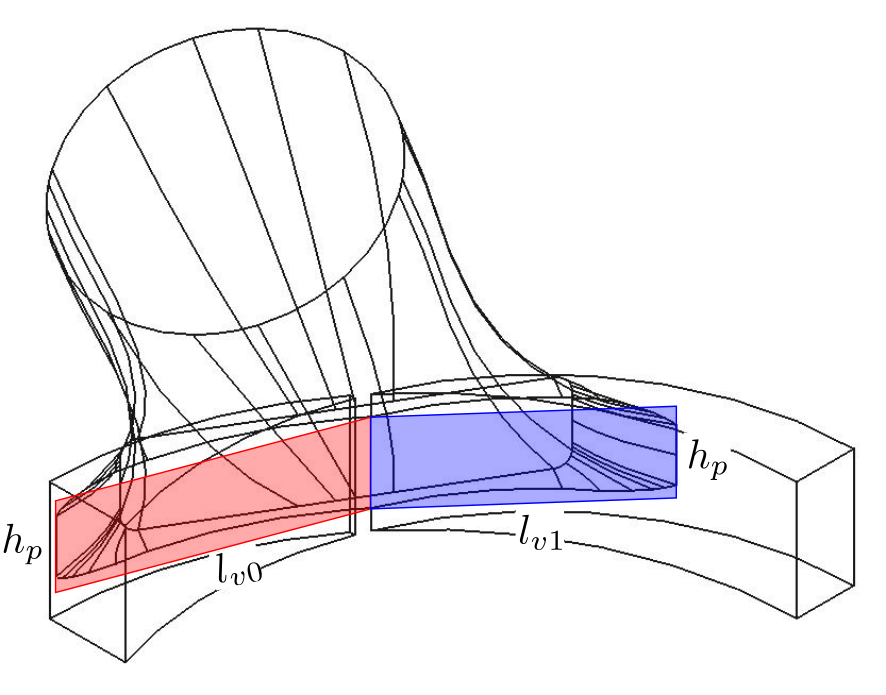
\includegraphics[]{area_referencia.png}
    \caption{Área de referencia}
    \label{fig:area_referencia}
\end{figure}

Los valores de densidad, velocidad, presión y temperatura se obtienen de los
datos de salida de ICESym para un puerto, ángulo y velocidad dada, en
particular del archivo de salida con nombre \emph{$cyl_0.txt$} que contiene
información relevante a la cámara de combustión.
%
Para la temperatura se utiliza la temperatura de cámara, $T_0 = T_C$, la
presión antes y después del puerto se selecciona de acuerdo al sentido de
flujo, en caso de ser flujo hacia la cámara de combustión, la presión en el
puerto se utiliza como inicial $P_0$ y la presión en la cámara es la
aproximación a la presión en la restricción $P_T$.

Para inicializar el campo de presión y densidades, se usa la media entre las
cámaras que se estén simulando y se establerce un campo uniforme.

La velocidad se incicializa con un campo nulo de velocidades, que en la
configuración de OpenFOAM se designa como \emph{internalField uniform (0 0 0)}.

En resumen, los valores iniciales de los campos de presión, temperatura y velocidad

\begin{table}
\centering
    \begin{tabular}{cccc} \toprule
        Var & Campo         & Parche                      & Pared \\
        T   & uniforme T0   & inletOutlet                 & uniforme T9\\ \midrule
        P   & uniform Pavg  & uniformTotalPressure        & Pi \\
        U   & uniform (0 0 0) & pressureInletOutletVelocity & valor fijo(0 0 0)\\
        rho & uniform rhoAvg \\ \bottomrule
    \end{tabular}
    \caption{Condiciones iniciales} \label{tab:cc}
\end{table}

En todos los casos se tomará como velocidad de referencia a la media entre la
velocidad en la punta del tubo de las cámaras solapadas.
%
Del mismo modo, la temperatura será la temperatura de cámara media.

Si hay o no solape de cámaras va a depender tanto de la geometría del puerto
como de la posición del ciclo en la que se encuentre, para determinar las
condiciones iniciales se debe tener en cuenta el solape.
%
En la figura \ref{fig:geom} se muestra un corte del puerto con un plano cuya
normal está en $\vec{z}$, se denominará a la cámara que esté a la izquierda
como cámara 0 y a la que esté a la derecha cámara 1
%
Al haber solape de cámaras, para definir la presión del puerto y estimar las
condiciones iniciales de los parámetros viscosos que requiere el modelo
$k-\epsilon$ se utilizan valores medios de presión, velocidad y temperatura de
ambas cámaras.
%
Además, las condiciones inicales de que se aplican al parche denominado
\emph{puerto} es igual a la media aritmética de la velocidad de las velocidades
de los puertos de ambas cámaras, Lo mismo sucede con la presión, densidad y
temperatura.

A partir de estos datos se calculan varias propiedades termodinámicas del gas,
incluyendo la constante del gas, masa molar, viscosidad cinemática y demás.
%
Para calcular estas propiedades se asume que el gas no contiene gases
residuales.

Finalmente el caudal másico yse obtiene con OpenFOAM, en donde se simula el
tiempo suficiente para que los caudales másicos por entradas o salidas se
estabilice, como se ve en la figura \ref{fig:caudalMasico}.

\begin{figure}
    \centering
    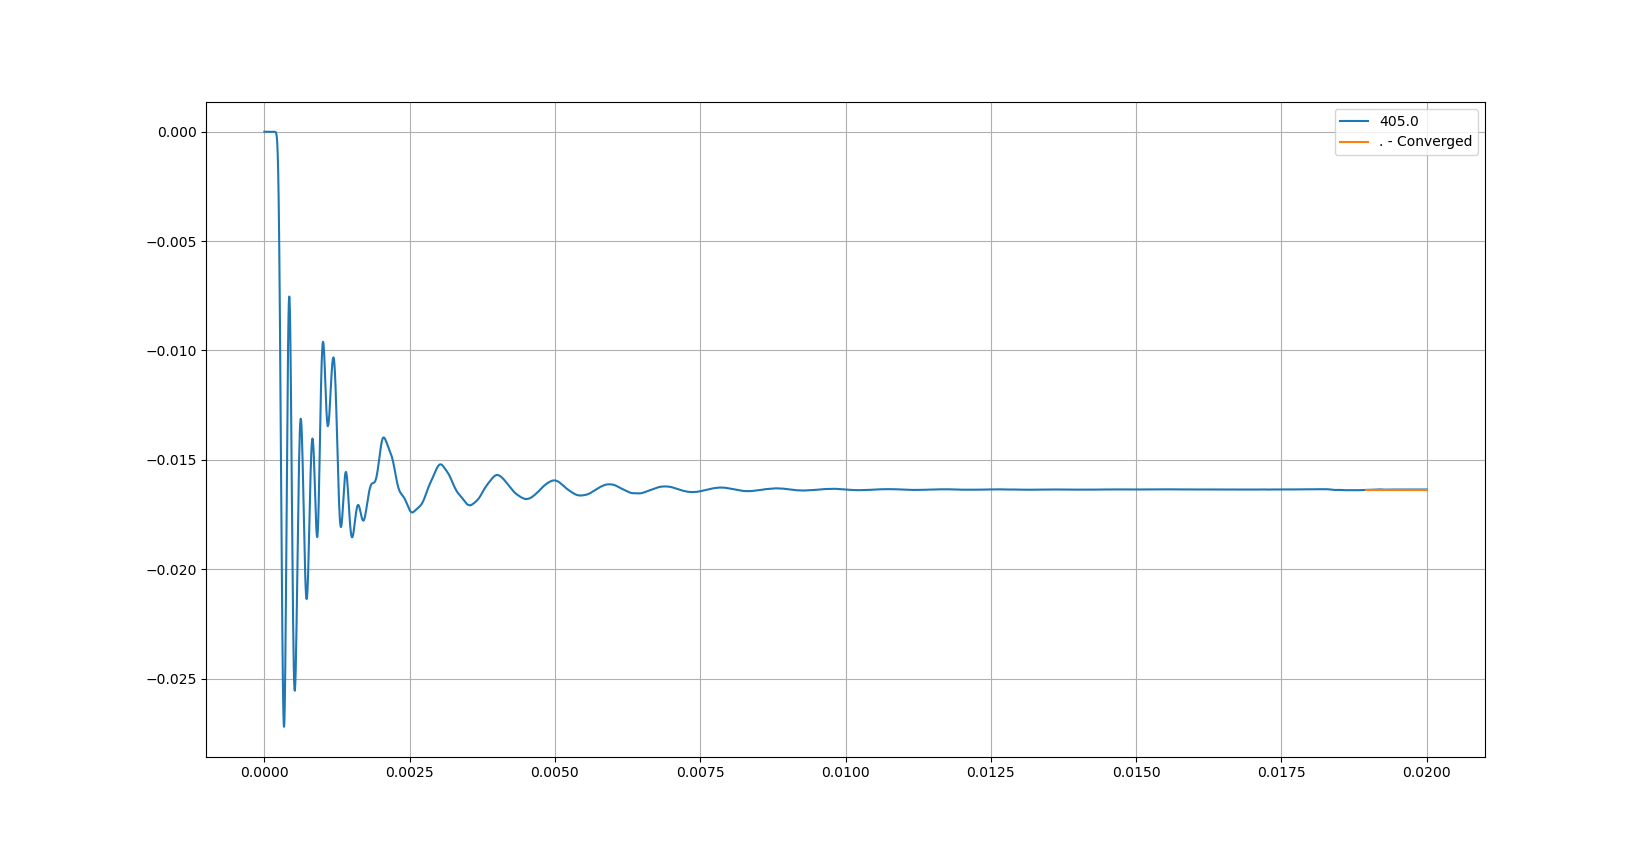
\includegraphics[width=0.6\textwidth]{surfaceFieldValue_405.0.png}
    \caption{Flujometrías para el puerto de Admisión}
    \label{fig:caudalMasico}
\end{figure}
En todos los casos se tomará como velocidad de referencia a la media entre la
velocidad en la punta del tubo de las cámaras que se estén solapando.
%
Del mismo modo, la temperatura será la temperatura de cámara media.

Si hay o no solape de cámaras va a depender tanto de la geometría del puerto
como de la posición del ciclo en la que se encuentre, para determinar las
condiciones iniciales se debe tener en cuenta el solape.
%
En la figura \ref{fig:geom} se muestra un corte del puerto con un plano cuya
normal está en $\vec{z}$, se denominará a la cámara que esté a la izquierda
como cámara 0 y a la que esté a la derecha cámara 1
%
Al haber solape de cámaras, para definir la presión del puerto y estimar las
condiciones iniciales de los parámetros viscosos que requiere el modelo
$k-\epsilon$ se utilizan valores medios de presión, velocidad y temperatura de
ambas cámaras.
%
Además, las condiciones inicales de que se aplican al parche denominado
\emph{puerto} es igual a la media aritmética de la velocidad de las velocidades
de los puertos de ambas cámaras, Lo mismo sucede con la presión, densidad y
temperatura.


\subsection{Mapa de $C_D$}
%
Para obtener el mapa se tomaran valores de flujo másico en las combinaciones de
$(\Delta P, l_v)$ que están indicadas en la tabla \ref{tab:casos}.
%
% En la figura \ref{fig:flujometrias} se ve que se eligieron más cantidad de
% muestreos en las zonas donde hay mayores cambios de presión.
%
% La figura \ref{fig:flujometrias} fué obtenida a partir de los resultados del
% simulador ICESym, restando para las velocidades seleccionadas la presión de la
% cámara a la presión en la boca del puerto.

\begin{figure}
    \centering
    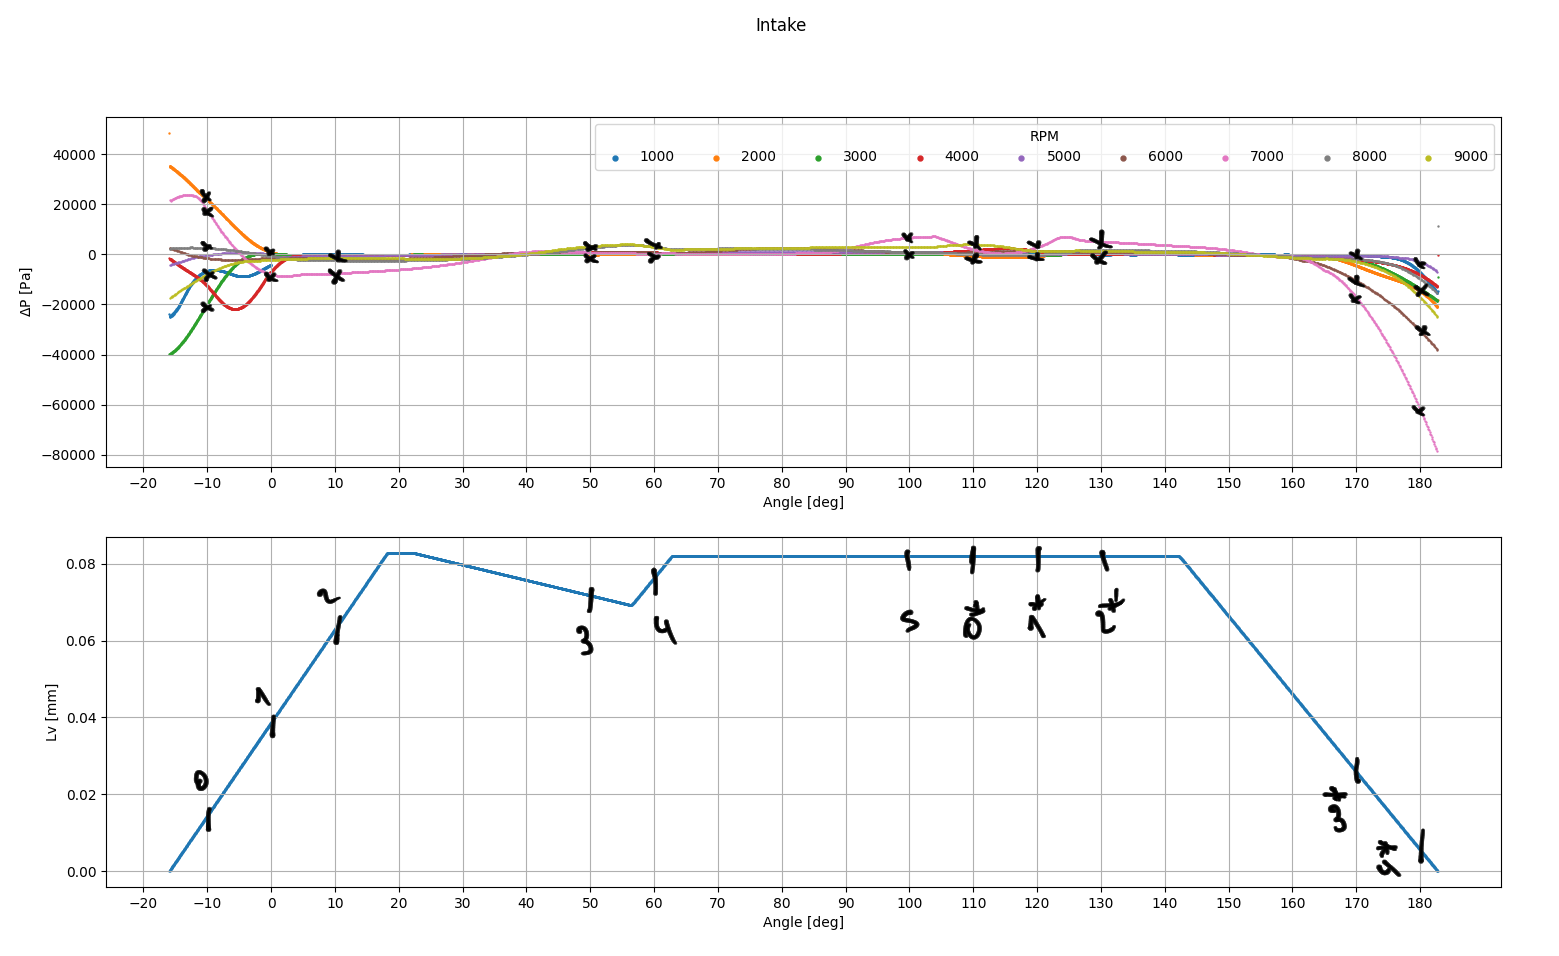
\includegraphics[width=1\textwidth]{flujometrias_admision.png}
    \caption{Flujometrías para el puerto de Admisión}
    \label{fig:flujometrias}
\end{figure}

\begin{table}
    \centering
    \begin{tabular}{rll} \toprule
        Caso & Ángulos  & Velocidades (rpm) \\ \midrule
        0    & -10, 110 & 1000, 2000, 3000, 7000, 8000 \\
        1    & 0, 120   & 2000, 7000 \\
        2    & 10, 130  & 2000, 7000 \\
        3    & 50, 170  & 3000, 7000, 9000 \\
        4    & 60, 180  & 3000, 5000, 6000, 7000 \\
        5    & 95       & 1000, 7000\\ \bottomrule
    \end{tabular}
    \caption{Flujometrías a realizar}
    \label{tab:casos}
\end{table}

Como se ve en la Figura \ref{fig:flujometrias}, los puntos a evaluar son los
listados en la Tabla \ref{tab:casos}.



\begin{figure}[h]
    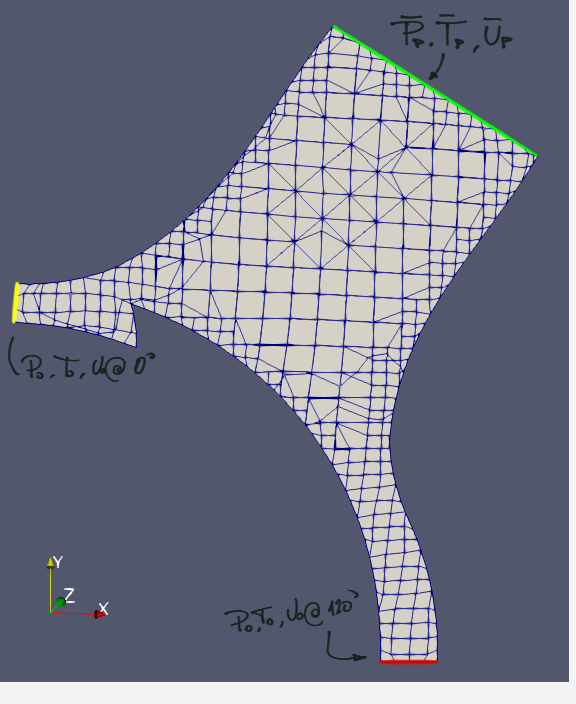
\includegraphics[width=0.8\textwidth]{caso_1-cc.png}
    \caption{Condiciones de borde}
    \label{fig:geom}
\end{figure}

Dentro del volumen de control, el campo de presiones se inicializa con el valor
medio de presiones de las cámaras y el campo de velocidades se hace
inicialmente (0,0,0).

\section{Estudio de convergencia de malla}
%
Para generar la malla primero se representa el volumen a simular con freecad,
procesada con slaome para obtener un conjunto de parches en formato ASCII stl
que puede ser procesado por snappyHexMesh.

snappyHexMesh requiere de una malla inicial para poder comenzar a tabajar, esta
se genera con la aplicaicón blockMesh



%Un estudio de convergencia de malla es una herramienta para evaluar los errores
%de discretización espacial de un estudio de CFD y consiste básicamente en:

%\begin{enumerate}
%    %
%    \item Seleccionar un indicador del tamaño de malla $h$.
%    %
%    \item Elegir un indicador de la convergencia de malla $f$, suele ser la
%        variable de estudio.
%    %
%    \item Seleccionar un coeficiente de refinamiento $r$ y realizar al menos 2
%        simulaciones, manteniendo $r$ constante.
%    %
%    \item Calcular el orden de convergencia de la serie de datos $p$.
%    %
%    \item Estimar $f_{h=0}$
%    %
%    \item Calcular el Índice de Convergencia de Malla (GCI por sus siglas en
%        inglés).
%    %
%    \item Comprobar que se está dentro del rango asintótico de convergencia.
%    %
%\end{enumerate}

%El error de discretización surge de aplicar las ecuaciones de gobierno a un
%dominio espacial discreto (la malla).
%%
%A medida que se reduce el tamaño de celda, el resultado del estudio de CFD se
%vuelve menos sensible a mayores refinamientos y es esperable que el error de
%discretización tienda asintóticamente a cero cuando el tamaño de la malla
%tiende a cero.

%En la Figura \ref{fig:flujometrias} y la Tabla \ref{tab:casos} se indican los
%puntos donde se va a ensayar el puerto de admisión con el fin de obtener el
%valor de caudal másico o volumétrico que fluja por el puerto en distintas
%posiciones del rotor y a distintas velocidades de rotación.
%%
%Dada la cantidad de flujometrías a realizar se opta por realizar el estudio de
%convergencia solo en algunos de los casos, los cuales serán utilizados como
%referencia e indicarán el nivel mínimo de refinamiento mínimo necesario a
%utilizar para todos los casos.

%% Se utilizará el mismo paso tempral en todos los refinamientos.

%\begin{sidewaysfigure}
%    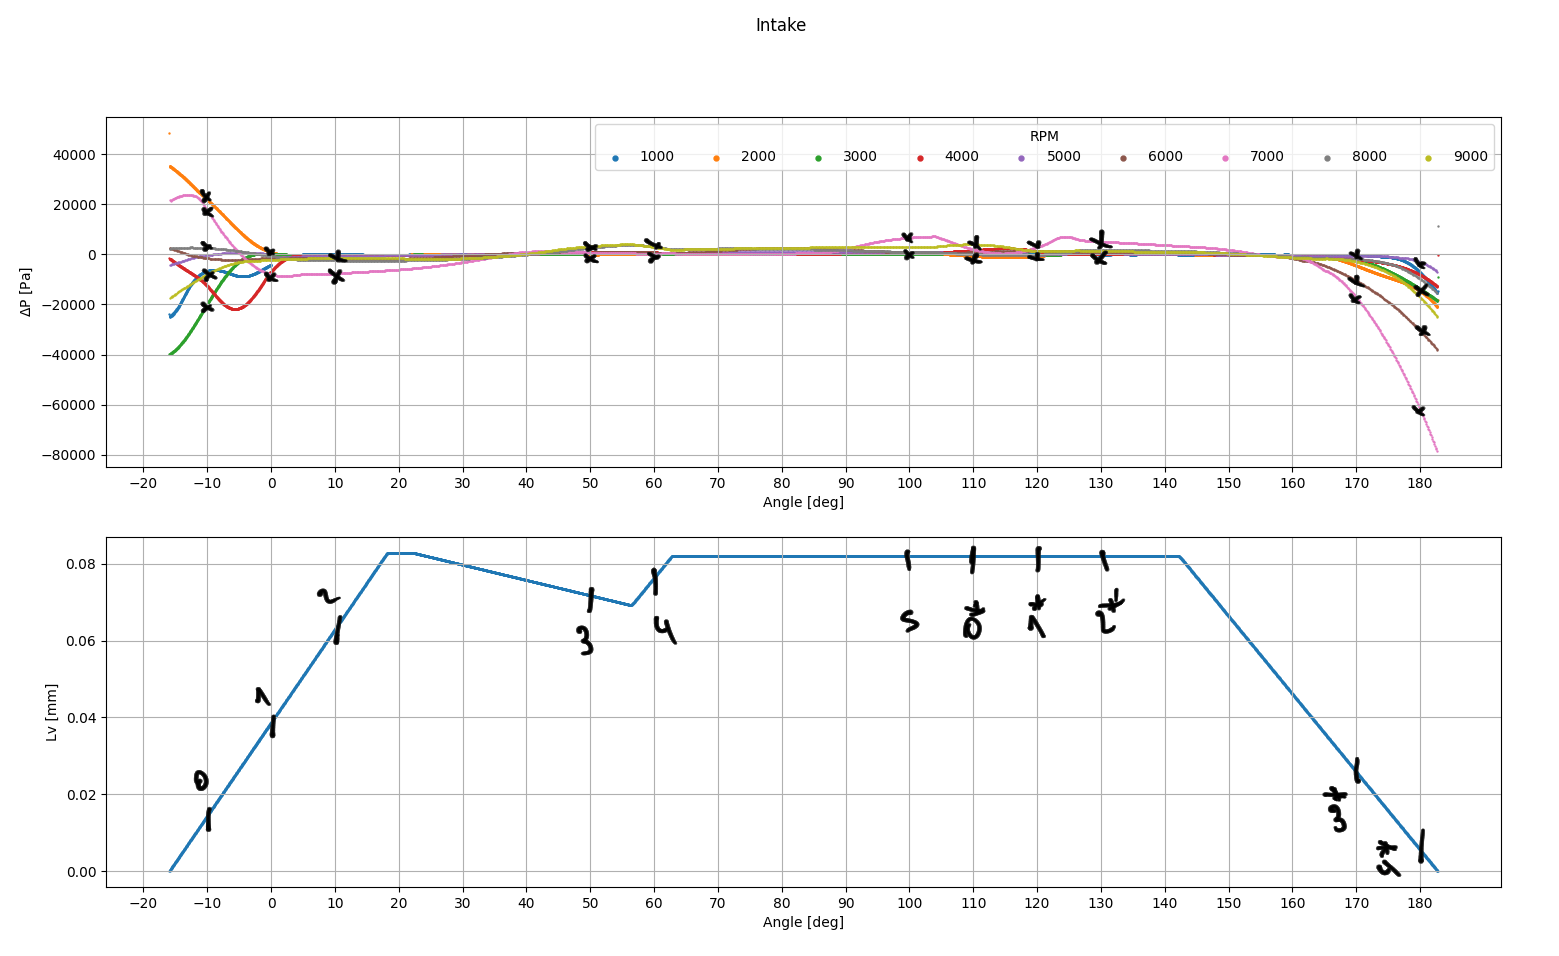
\includegraphics[width=1\textwidth]{flujometrias_admision.png}
%    \caption{Flujometrías para el puerto de admisión}
%    \label{fig:flujometrias}
%\end{sidewaysfigure}

%\begin{table}
%    \centering
%    \begin{tabular}{rcc} \toprule
%        Caso & Ángulos & Velocidades (rpm) \\ \midrule
%        0 & -10, 110 & 1000, 2000, 3000, 7000, 8000\\
%        1 & 0, 120 & 2000, 7000\\
%        2 & 10, 130 & 2000, 7000\\
%        3 & 50, 170 & 3000, 7000, 9000\\
%        4 & 60, 180 & 3000, 5000, 6000, 7000\\
%        5 & 95 & 1000, 7000\\ \bottomrule
%    \end{tabular}
%    \caption{Flujometrías para el puerto de admisión}
%    \label{tab:casos}
%\end{table}

%Hay que distinguir en entre los refinamientos necesarios de flujometrías en
%régimen compresible e incompresible, los casos a tomar como referencia son el
%0, 4 y 5.

%\subsection{Selección de $h$, $r$ y $f$}
%%
%El procedimiento para generar la malla consiste en crear una malla inicial con
%la utilidad \emph{blockMesh} la cual es un punto de partida de
%\emph{snappyHexMesh}.
%%
%Se busca que la malla creada por \emph{blockMesh} este compuesta por celdas
%cúbicas, como se ilustra en la Figura \ref{fig:celdas_bm} el lado de estas
%celdas es el que se toma como indicador del tamaño de malla $h$.
%%
%El coeficiente de refinamiento es el cociente entre el tamaño $h$ de dos pasos
%de refinamiento, como se indica en la ecuación \ref{eq:r}, el mismo se toma
%igual a 1.5 y se mantiene constante para todos los refinamientos.
%%
%Se realizarán refinamientos con mallas de $11.25mm \rightarrow 7.5mm
%\rightarrow 5mm$.

%\begin{equation}
%    \label{eq:r}
%    r = \frac{h_{i+1}}{h_{i}} = 1.5
%\end{equation}


%\begin{figure}[h]
%    \centering
%    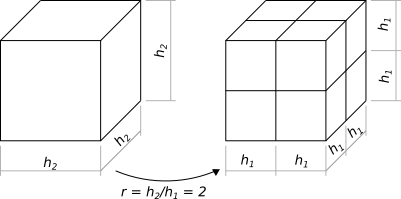
\includegraphics{celdas_block_mesh.png}
%    \caption{Refinamiento con $r=2$}
%    \label{fig:celdas_bm}
%\end{figure}

%Para verificar la convergencia de malla se utiliza el flujo másico a través
%de las superficies definidas como entrada/salida de cámaras.
%%
%En la figura \ref{fig:parches} se indican las superficies por las cuales hay
%flujo másico, siempre que haya solape de cámaras, la cámara que esté a la
%izquierda será llamada cámara 0 y la que esté a derecha cámara 1.
%%
%La superficie que indica la conexión entre el puerto y el resto de los conductos
%de intercambio de gases se denominará puerto.


%En caso de flujo presente un $Ma < 0.3$, el \emph{solver} a utilizar devuelve
%el flujo volumétrico, por lo que se usa este como indicador en lugar del flujo
%másico.

%\begin{figure}[ht]
%    \centering
%    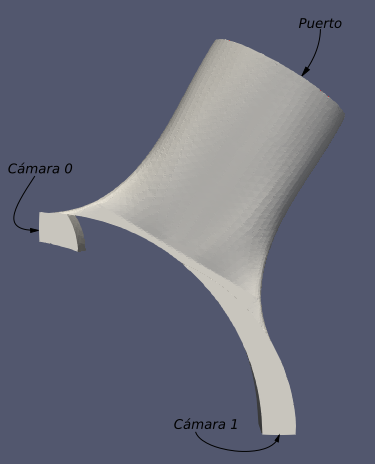
\includegraphics[width=0.4\textwidth]{nombres-parches.png}
%    \caption{Vista superior del volumen de control}
%    \label{fig:parches}
%\end{figure}

%\subsection{Orden de convergencia}
%%
%El orden de convergencia $p$ indica que tan rápido se acerca una secuencia a un
%límite.
%%
%Una secuencia ${x_n}$ que converge a $x^*$ tiene orden de convergencia $p \ge
%1$ y constante asintótica de error $\mu$.

%\begin{equation}
%    \lim_{n\rightarrow \infty} \frac{|x_{n+1} - x^*|} {|x_{n} - x^*|^p} = \mu
%\end{equation}

%El orden de convergencia se puede obtener de comparando el comportamiento del
%error, definido como la diferencia ente la solución exacta o del continuo y la
%discreta.

%\begin{equation}
%    E = f(h) - f_{exacta} = Ch^p + \xi
%    \label{eq:1}
%\end{equation}

%Dónde $C$ es una constante, $h$ es una medida del nivel de refinamiento de la
%malla, $p$ es el orden de convergencia y $\xi$ son términos de orden superior.
%%
%Despreciando los términos de orden superior $\xi$ y tomando logaritmo a ambos
%lados, se puede expresar la ecuación \ref{eq:1} como:

%\begin{equation}
%    \log(E) = \log(C) + p \cdot \log(h)
%\end{equation}

%De esta forma $p$ es la pendiente de la curva de $\log(E)=f(\log(h))$ y
%conociendo al menos 3 puntos puede calcular $p$ como:

%\begin{equation}
%p = \ln \left( \frac{ f_3 - f_2 } { f_2 - f_1 } \right) / \ln(r)
%\label{eq:ord-conv}
%\end{equation}

%\subsection{Resultado ''exacto``}
%%
%El resultado de una simulación numérica se puede expresar de forma general
%como:

%\begin{equation} \label{eq:expansion}
%    f = f_{h=0} + g_1 h + g_2 h^2 + g_3 h^3 + ...
%\end{equation}

%Dónde $h$ es el tamaño de la malla y $g_1$, $g_2$ y $g_3$ son funciones
%independientes $h$, la cantidad $f$ es considerada de segundo orden si $g1 =
%0$.
%%
%El valor de $f_{h=0}$ es el resultado que tendría la simulación con una malla
%infinitamente fina, $h \rightarrow 0$.

%\section{Índice de convergencia de malla}
%%
%El índice de convergencia de malla o GCI por sus siglas en inglés es una forma
%de reportar los resultados de convergencia de malla, es un indicador de qué tan
%lejos se encuentran los resultados obtenidos del resultado numérico exacto
%($f_{h=0}$) y surge de la siguiente ecuación:

%\begin{equation} \label{eq:gci}
%GCI_{i \rightarrow j} = \frac{F_S |\epsilon|}{r^p - 1}
%\end{equation}

%Dónde:
%\begin{description}
%    \item[$F_S$] es un factor de seguridad, se toma 1.25.
%    \item[$\epsilon$] es el error relativo $\epsilon = (f_i - f_j) / f_j$
%    \item[$r$] es el factor de refinamiento $r = h_i/h_j$
%    \item[$p$] es el orden de convergencia relativo a los pasos i, j
%\end{description}

%De este modo, si para un nivel de refinamiento $h_i$ la simulación da como
%resultado un valor $x_i$ con $GCI_i$ dado, se puede decir que el resultado
%de la simulación es $x_i \pm GCI_i \cdot 100$.
%%
%Se tomará como GCI aceptable o banda de error un valor cercano a 5\%.

\section{Resultados}

Para determinar el tipo de \emph{solver} a utilizar se hace una primer corrida
de cada caso asumiendo que el flujo se puede asumir como incompresible, es
decir, que el número de Mach máximo del caso convergido va a ser menor a 0.3.
%
Estos resultados no son definitivos en cuanto al \emph{solver} a utilizar,
puede suceder que a medida que refine un caso el $Ma$ aumente, en cuyo caso
se deberá evaluar si es necesario revisar la hipótesis de flujo incompresible.

% ESe dice que el caso converge cuando el flujo másico a través de cualquiera de
% las entradas/salidas del dominio se estabiliza.

El caso se ejecuta hasta obtener una convergencia del caudal másico para todas
las cámaras involucradas en la simulación, inicialmente este tiempo es de 0.01
segundos.
%
El objetivo de cada flujometría es obtener un valor de caudal másico, para esto
se modelo cada puerto en distintas posiciones y velocidades de rotación.
%
Como se mencionó,los valores iniciales se determinan a partir de los datos de
salida del simulador, con un script de nombre \emph{pre.py} que es un compilado
de funciones para determinar propiedades termodinámicas de las mezclas de gases
quemados o no quemados.

Con esto se obtiene un mapa de caudales másicos que se utilizan para calcular
el coeficiente de descarga con el uso de un script de nombre \emph{post.py}.


En las imágenes que siguen se muestan el campo de velocidades de un corte de
algunos puntos del mapa obtenido.


El mapa de $C_D$ es un conjunto finito de puntos, estos se utilizan para crear
una superficie mediante el método de interpolación de punto más cercano con
suavizamiento.

Los puntos obtenidos se listan en la tabla xxx y la superficie correspondiente
en la figura xxx.

\begin{table}
    \centering
    \begin{tabular}{rll}\toprule
        Caso & Velocidad [RPM] & $Ma_{max}$ \\ \midrule
        0 & 1000 & 0.29 \\
        0 & 2000 & 0.65 \\
        0 & 3000 & 0.49 \\
        0 & 7000 & 0.65 \\
        0 & 8000 & 0.23 \\
        1 & 2000 & 0.14 \\
        1 & 7000 & 0.4 \\
        2 & 2000 & 0.1 \\
        2 & 7000 & 0.43 \\
        3 & 3000 & 0.16 \\
        3 & 7000 & 0.37 \\
        3 & 9000 & 0.24 \\
        4 & 3000 & 0.35 \\
        4 & 5000 & 0.38 \\
        4 & 6000 & 0.49 \\
        4 & 7000 & 0.63 \\
        5 & 1000 & 0.01 \\
        5 & 7000 & 0.45 \\ \bottomrule
    \end{tabular}
    \caption{Números de Mach}
    \label{tab:mach}
\end{table}

\section{Caso 0 - 1000rpm}

El caso simulado tiene solape de cámaras, una a $-10^{\circ}$ y otra a
$110^{\circ}$, con el motor girando a 1000 RPM.
%
El flujo se modela como incompresible\footnote{Ver Tabla \ref{tab:mach}}, la
geometría del caso y la ubicación de los parches correspondientes a la cámara
0, 1 y a la "boca" del puerto.

\begin{figure}
    \centering
    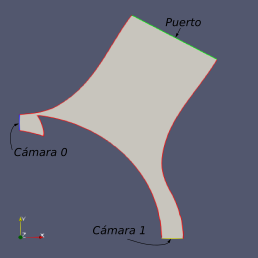
\includegraphics{caso0.png}
    \caption{Geometría a modelar}
    \label{fig:caso0}
\end{figure}

\begin{table}
    \centering
    \begin{tabular}{rll}\toprule
        Parámetro & Valor \\ \midrule
        $\theta_0\ [^{\circ}]$ & 590 \\
        $\theta_1\ [^{\circ}]$ & 110 \\
        $\epsilon_{est}$ & 195.467 \\
        $\gamma_{est}$ & 1.309 \\
        $\kappa_{est}$ & 1.364471 \\
        $\nu_{est}$ & 4.3e-05 \\
        $p_0 [Pa]$ & 107355.2 \\
        $p_1 [Pa]$ & 100867.47 \\
        $\overline{p} [Pa]$ & 104111.33 \\
        $\overline{p_{puerto}} [Pa]$ & 100780.23 \\
        $\overline{\rho} [kg/m^3]$ & 0.643938 \\
        $\overline{T} [K]$ & 589.89 \\ \bottomrule
    \end{tabular}
    \caption{Valores iniciales}
    \label{tab:caso0_ci}
\end{table}


En la tabla \ref{tab:res_caso0}se muestran los resultados de 3 pasos de
refinamiento. TENGO QUE REHACER TODOS EN RÉGIMEN COMPRESIBLE

\begin{table}
    \centering
    \begin{tabular}{rccccc}\toprule
        h [mm] & $h_{norm}$ & $N^{\circ}$ celdas & $Ma$ & $\dot{V_{0}}\ [m^3/s] $ & $\dot{V_{1}}\ [m^3/s]$ \\ \midrule
        5      & 1.0        & 167900             & 0.36 & -0.006312     & -0.012329 \\
        10     & 2.0        & 52210              & 0.33 & -0.006455     & -0.011692 \\
        20     & 4.0        & 20795              & 0.29 & -0.006668     & -0.011652 \\ \bottomrule
    \end{tabular}
    \caption{Flujos volumétricos para ambas cámaras}
    \label{tab:res_caso0}
\end{table}

Con estos datos se puede calcular el orden de convergencia y el resultado
extrapolado a $h=0$.

\begin{table}
    \centering
    \begin{tabular}{rcc}\toprule
        Parámetro & Cámara 0  & Cámara 1  \\ \midrule
        p         &  0.565833 & -3.967099 \\
        $f_{h=0}$ & -0.006013 & -0.011649 \\ \bottomrule
    \end{tabular}
    \caption{Orden de convergencia y resultado exacto}
    \label{tab:res1_caso0}
\end{table}

Y con el orden de convergencia se pueden calcular los valores de GCI.

\begin{table}
    \centering
    \begin{tabular}{rccc}\toprule
        Paso              & $r$ & $GCI_0(\%)$ & $GCI_1(\%)$ \\ \midrule
        1 $\rightarrow$ 2 & 2   & -5.923628   & 6.895404 \\
        2 $\rightarrow$ 3 & 2   & -8.573288   & 0.464910 \\ \bottomrule
    \end{tabular}
    \caption{GCI}
    \label{tab:gci_caso_0}
\end{table}

Con estos resultados se verifica que se esté en rango de convergencia
asintótica, como se indica en la Tabla \ref{tab:rac_caso_0}, los flujos
másicos de ambas cámaras se encuentran en rango de convergencia asintótica.

\begin{table}
    \centering
    \begin{tabular}{rccc}\toprule
        Rango               & $rac_0$  & $rac_1$ \\ \midrule
        12 $\rightarrow$ 23 & 1.022758 & 0.948364 \\ \bottomrule
    \end{tabular}
    \caption{Verificación de convergencia}
    \label{tab:rac_caso_0}
\end{table}


\section{Caso 0 - 7000 rpm}

\section{Caso 4 - 7000 rpm}

\section{Caso 5 - 1000rpm}

El caso simulado tiene una sola cámara a $100^{\circ}$ del ciclo, con el motor
girando a 1000 RPM.
%
El flujo se modela como incompresible\footnote{Ver Tabla \ref{tab:mach}}, la
geometría del caso y la ubicación de los parches correspondientes a la cámara
0, 1 y a la "boca" del puerto.

\begin{figure}
    \centering
    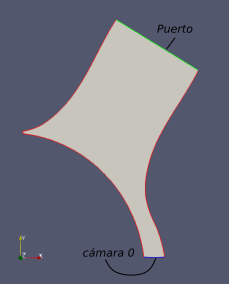
\includegraphics{caso5.png}
    \caption{Geometría a modelar}
    \label{fig:caso5}
\end{figure}

\begin{table}
    \centering
    \begin{tabular}{rll}\toprule
        Parámetro & Valor \\ \midrule
        $\theta_0\ [^{\circ}]$ & 100 \\
        $\epsilon_{est}$ & 25.271765 \\
        $\gamma_{est}$ & 1.329 \\
        $\kappa_{est}$ & 0.348878 \\
        $\nu_{est}$ & 2.9e-05 \\
        $\overline{p} [Pa]$ & 103732.67 \\
        $\overline{p_{puerto}} [Pa]$ & 103773.09 \\
        $\overline{\rho} [kg/m^3]$ & 0.797554 \\
        $\overline{T} [K]$ & 453.18 \\ \bottomrule
    \end{tabular}
    \caption{Valores iniciales}
    \label{tab:caso5_ci}
\end{table}

En la tabla \ref{tab:res_caso5} se muestran los resultados de 3 pasos de
refinamiento.

\begin{table}[h]
    \centering
    \begin{tabular}{rcccc}\toprule
        h [mm] & $h_{norm}$ & $N^{\circ}$ celdas & $Ma$ & $\dot{V}\ [m^3/s]$ \\ \midrule
        5      & 1.0        & 167900             & 0.36 & -0.006312 \\
        10     & 2.0        & 52210              & 0.33 & -0.006455 \\
        20     & 4.0        & 20795              & 0.29 & -0.006668 \\ \bottomrule
    \end{tabular}
    \caption{Flujos volumétricos para ambas cámaras}
    \label{tab:res_caso5}
\end{table}

Con estos datos se puede calcular el orden de convergencia y el resultado
extrapolado a $h=0$.

\begin{table}[h]
    \centering
    \begin{tabular}{rc}\toprule
        Parámetro & Cámara 0  \\ \midrule
        p         &  0.565833 \\
        $f_{h=0}$ & -0.006013 \\ \bottomrule
    \end{tabular}
    \caption{Orden de convergencia y resultado exacto}
    \label{tab:res1_caso5}
\end{table}

Y con el orden de convergencia se pueden calcular los valores de GCI.

\begin{table}
    \centering
    \begin{tabular}{rcc}\toprule
        Paso              & $r$ & $GCI_0(\%)$ \\ \midrule
        1 $\rightarrow$ 2 & 2   & -5.923628   \\
        2 $\rightarrow$ 3 & 2   & -8.573288   \\ \bottomrule
    \end{tabular}
    \caption{GCI}
    \label{tab:gci_caso_5}
\end{table}

\begin{table}
    \centering
    \begin{tabular}{rccc}\toprule
        Rango               & $rac_0$  \\ \midrule
        12 $\rightarrow$ 23 & 1.022758 \\ \bottomrule
    \end{tabular}
    \caption{Verificación de convergencia}
    \label{tab:rac_caso_5}
\end{table}

Con estos resultados se verifica que se esté en rango de convergencia
asintótica, como se indica en la Tabla \ref{tab:rac_caso_5}, los flujos
másicos de ambas cámaras se encuentran en rango de convergencia asintótica.
